% !Rnw weave = knitr
% !TeX program = pdfLaTeX
\documentclass[a4paper,10pt]{article}\usepackage[]{graphicx}\usepackage[]{xcolor}
% maxwidth is the original width if it is less than linewidth
% otherwise use linewidth (to make sure the graphics do not exceed the margin)
\makeatletter
\def\maxwidth{ %
  \ifdim\Gin@nat@width>\linewidth
    \linewidth
  \else
    \Gin@nat@width
  \fi
}
\makeatother

\definecolor{fgcolor}{rgb}{0.345, 0.345, 0.345}
\newcommand{\hlnum}[1]{\textcolor[rgb]{0.686,0.059,0.569}{#1}}%
\newcommand{\hlstr}[1]{\textcolor[rgb]{0.192,0.494,0.8}{#1}}%
\newcommand{\hlcom}[1]{\textcolor[rgb]{0.678,0.584,0.686}{\textit{#1}}}%
\newcommand{\hlopt}[1]{\textcolor[rgb]{0,0,0}{#1}}%
\newcommand{\hlstd}[1]{\textcolor[rgb]{0.345,0.345,0.345}{#1}}%
\newcommand{\hlkwa}[1]{\textcolor[rgb]{0.161,0.373,0.58}{\textbf{#1}}}%
\newcommand{\hlkwb}[1]{\textcolor[rgb]{0.69,0.353,0.396}{#1}}%
\newcommand{\hlkwc}[1]{\textcolor[rgb]{0.333,0.667,0.333}{#1}}%
\newcommand{\hlkwd}[1]{\textcolor[rgb]{0.737,0.353,0.396}{\textbf{#1}}}%
\let\hlipl\hlkwb

\usepackage{framed}
\makeatletter
\newenvironment{kframe}{%
 \def\at@end@of@kframe{}%
 \ifinner\ifhmode%
  \def\at@end@of@kframe{\end{minipage}}%
  \begin{minipage}{\columnwidth}%
 \fi\fi%
 \def\FrameCommand##1{\hskip\@totalleftmargin \hskip-\fboxsep
 \colorbox{shadecolor}{##1}\hskip-\fboxsep
     % There is no \\@totalrightmargin, so:
     \hskip-\linewidth \hskip-\@totalleftmargin \hskip\columnwidth}%
 \MakeFramed {\advance\hsize-\width
   \@totalleftmargin\z@ \linewidth\hsize
   \@setminipage}}%
 {\par\unskip\endMakeFramed%
 \at@end@of@kframe}
\makeatother

\definecolor{shadecolor}{rgb}{.97, .97, .97}
\definecolor{messagecolor}{rgb}{0, 0, 0}
\definecolor{warningcolor}{rgb}{1, 0, 1}
\definecolor{errorcolor}{rgb}{1, 0, 0}
\newenvironment{knitrout}{}{} % an empty environment to be redefined in TeX

\usepackage{alltt}
\usepackage[utf8]{inputenc}
\usepackage[T1]{fontenc}
\usepackage[french]{babel}
\usepackage{csquotes}
\usepackage{hyperref}
\usepackage{xcolor}

% Géométrie
\usepackage{geometry}
\geometry{
a4paper, 
total={170mm,257mm},
left=20mm,
top=15mm}

% Maths
\usepackage{amsmath}
\DeclareMathOperator*{\argmax}{argmax}
\DeclareMathOperator*{\argmin}{argmin}
\usepackage{amsfonts}
\usepackage{dsfont}
\usepackage{bm}

% Images 
\usepackage{wrapfig}
\usepackage{graphicx}
\graphicspath{ {./images/} }

% Citations et biblio
\usepackage[backend=biber, style=apa]{biblatex}
%== use and define color ==%
%\usepackage[style=numeric,backend=biber,doi=false,isbn=false,max
\AtEveryCite{\color{blue}}
\addbibresource{references.bib}


% Commande pour les nombres réels
\newcommand{\R}{\mathbb{R}}
\newcommand{\segspace}{\mathcal{T}_K}

% Commande pour les entiers naturels
\newcommand{\N}{\mathbb{N}}

% Commande pour les entiers relatifs
\newcommand{\Z}{\mathbb{Z}}

% Commande pour les nombres complexes
\newcommand{\C}{\mathbb{C}}

% Commande pour la probabilité
\newcommand{\Prob}{\mathbb{P}}

% Commande pour l'espérance
\newcommand{\E}{\mathbb{E}}

% Commande pour la variance
\newcommand{\Var}{\text{Var}}

% Commande pour la covariance
\newcommand{\Cov}{\text{Cov}}

% Commande pour la convergence en probabilité
\newcommand{\convprob}{\xrightarrow{P}}

% Commande pour la convergence en loi
\newcommand{\convloi}{\xrightarrow{d}}

% Commande pour la convergence en moyenne quadratique
\newcommand{\convmq}{\xrightarrow{L^2}}

% Poisson
\newcommand{\Poisson}[1]{\mathcal{P} ({#1})}

% Pagination
\usepackage{fancyhdr}
\pagestyle{fancy}
% Place Page X of Y on the right-hand
% side of the footer
\fancyhf{}
\rfoot{\thepage}

\title{\vspace{-1.5cm}\large Détection de ruptures dans des processus de Poisson - Stéphane Robin\\
\small Compte-rendu du séminaire\vspace{-0.5cm}}
\date{\small 30 Jan. 2024}
\author{\small Louis Lacoste}



\IfFileExists{upquote.sty}{\usepackage{upquote}}{}
\begin{document}
\maketitle

\section{Introduction}

Stéphane Robin nous présente une méthode qu'ils ont développé avec Emilie Lebarbier
et Charlotte Dion-Blanc. Cette méthode est présentée dans l'article 
\cite{dion-blancDetectionRupturesMultiples2023} sur HAL.

\begin{wrapfigure}{l}{0.35\textwidth}
    \centering
    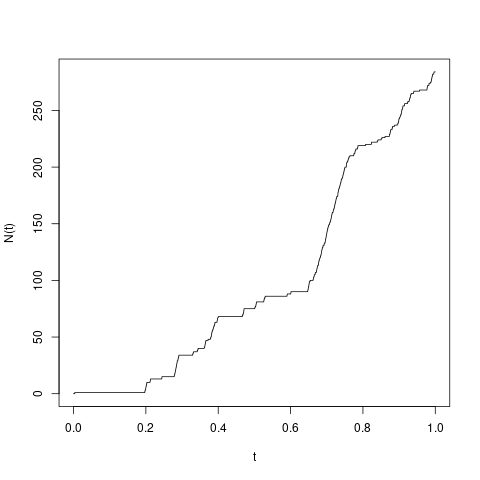
\includegraphics[width=0.35\textwidth]{graph-cris-chauve-souris}
    \caption{Comptage de cris de chauve-souris (nuit du 17 juillet 2019)}
    \label{fig:graph-cris-chauve-souris}
\end{wrapfigure}

La méthode considère des données de comptages au cours du temps. Un exemple de 
telles données est celui du nombre de cris de chauve-souris au cours de la nuit.
Ces données sont présentées dans sur la figure~\ref{fig:graph-cris-chauve-souris}.
Ou encore les données d'éruption du volcan Kilauea présentée sur la figure~\ref{fig:graph-eruption-kilauea}.

\begin{wrapfigure}{r}{0.35\textwidth}
    \centering
    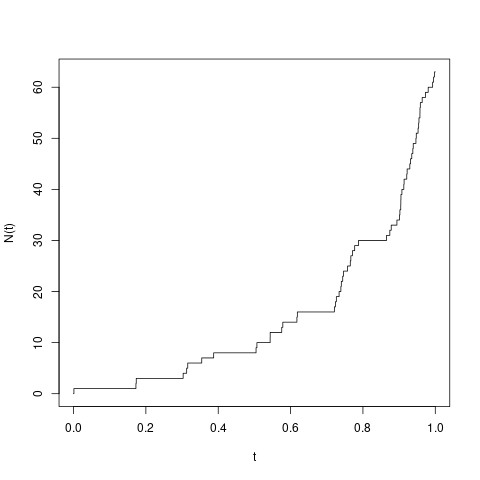
\includegraphics[width=0.35\textwidth]{graph-eruption-kilauea}
    \caption{Données d'éruption du Kilauea, 1750 - 1984}
    \label{fig:graph-eruption-kilauea}
\end{wrapfigure}

L'intervalle de temps est normalisé, $t\in[0,1]$ et les instants d'évènements 
sont les $0<T_1<\dots T_i<\dots T_n < 1$.
Étant donné qu'il s'agit d'un comptage aléatoire, le processus \emph{naturel}
est le processus de comptage, $N(t) = \sum_{i=1}^n \mathds{1}_{T_i \leq t}$ et 
parmi les processus de comptage, le processus de Poisson défini par sa fonction d'intensité $\lambda(t)$.\\
\section{Méthode}

La méthode fait l'hypothèse que la fonction d'intensité est constante par 
morceaux et qu'il existe des \emph{points de ruptures} les $(\tau_k)_{0\leq k \leq K}$.
Et alors pour $t \in I_k = ] \tau_{k-1}; \tau_{k} ], \lambda(t) = \lambda_k$.
Ainsi l'objectif de la méthode est d'estimer les paramètres 
$\theta =((\tau_k)_{0\leq k \leq K}, (\lambda_k)_{0\leq k \leq K} )$ et de 
réaliser une \emph{sélection de modèle} pour obtenir le nombre de segments $K$.

\subsection{Segmentation}

Un rappel sur la segmentation en temps discret, nous montre que la programmation
dynamique permet ainsi de résoudre le problème d'estimation des paramètres dans 
ce cas qui semblait apparemment computationnellement complexe.

Dans le cas de la méthode, le problème d'optimisation est 
$$(\widehat{\bm{\tau}}, \widehat{\bm{\lambda}}) = 
\argmin_{\bm{\tau}\in\segspace, \bm{\lambda} \in (\R^+)^K} \gamma (\bm{\tau}, \bm{\lambda})$$

L'additivité du contraste: $\gamma(\bm\tau, \bm\lambda) = 
\sum_{k=1}^K C(\Delta N_k, \Delta\tau_k, \lambda_k)$ en tant que somme sur les 
segments aide à la résolution du problème d'optimisation.
En effet le $\bm \lambda = (\lambda_1, \dots, \lambda_K)$ optimal peut être obtenu grâce à la propriété d'additivité
en résolvant $\widehat \lambda_k = \lambda_k (\tau) = \argmin_{\lambda_k \in \R^+} 
C(\Delta N_k, \Delta\tau_k)$.
Et si la fonction de contraste est la log-vraisemblance négative, on a : 
$\widehat \lambda_k = \Delta N_k / \Delta \tau_k$.

Mais le problème difficile est celui de trouver le $\bm\tau = (\tau_0, \dots, 
\tau_K)$ optimal, car le problème 
d'optimisation est alors $\widehat \tau = 
\argmin_{\tau\in\segspace} \widehat \gamma(\tau), 
\widehat \gamma(\tau) = \gamma (\tau, \widehat \lambda (\tau))$ où $\segspace$ 
est l'espace de segmentation \textbf{continu}, $$\segspace = 
\bigl\{ \tau \in [0,1]^{K+1} : 0 = \tau_0 < \tau_1 \dots < \tau_{K-1} < 
\tau_K = 1 \bigr\}$$
Car le contraste n'est ni convexe ni continu par rapport à $\tau$.

\begin{wrapfigure}{l}{0.35\textwidth}
    \centering
    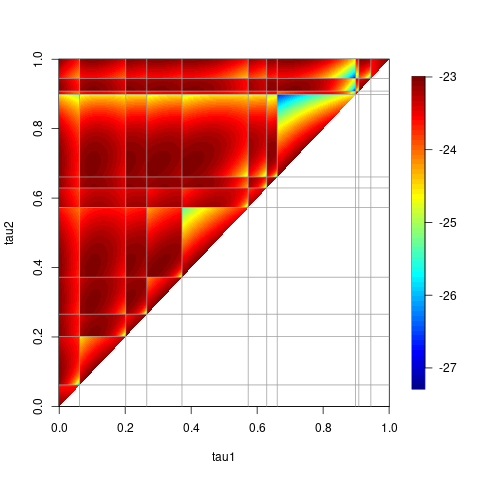
\includegraphics[width=0.35\textwidth]{contrast-function}
    \caption{Fonction de contraste pour $n=10$, $K=3$ et $\tau = (\tau_1,\tau_2)$}
    \label{fig:contrast-function}
\end{wrapfigure}

La figure~\ref{fig:contrast-function} présente les valeurs de la fonction de 
contraste pour les paramètres donnés. Sur la figure, chaque "bloc" correspond à
une partition des nombre d'évènements ($\Delta N = (\Delta N_1, \Delta N_2, 
\Delta N_3)$). 

L'idée est alors de partitionner le nombre d'évènements  $\mathcal{N} = 
\bigl\{ \nu \in \N^K : \sum_{k=1}^K \nu_k = n \bigr\}$ où $\nu_k$ est le nombre
d'évènements dans le segment k. Puis à partir de cette partition, on peut 
partitionner l'espace de segmentation $\mathcal{T}(\nu) = 
\bigl\{ \bm \tau \in \segspace : \Delta N = \nu \bigr\}$ qui satisfait la 
partition $\nu$. Ce qui permet de réécrire le problème de minimisation :
$$\min_{\bm{\tau}\in\segspace} \widehat \gamma (\bm{\tau}) = \min_{\nu \in 
\mathcal{N}^K} \min_{\bm{\tau}\in\mathcal{T}(\nu)} \widehat \gamma (\bm{\tau})$$
Et alors grâce au fait que

\begin{wrapfigure}{r}{0.35\textwidth}
    \centering
    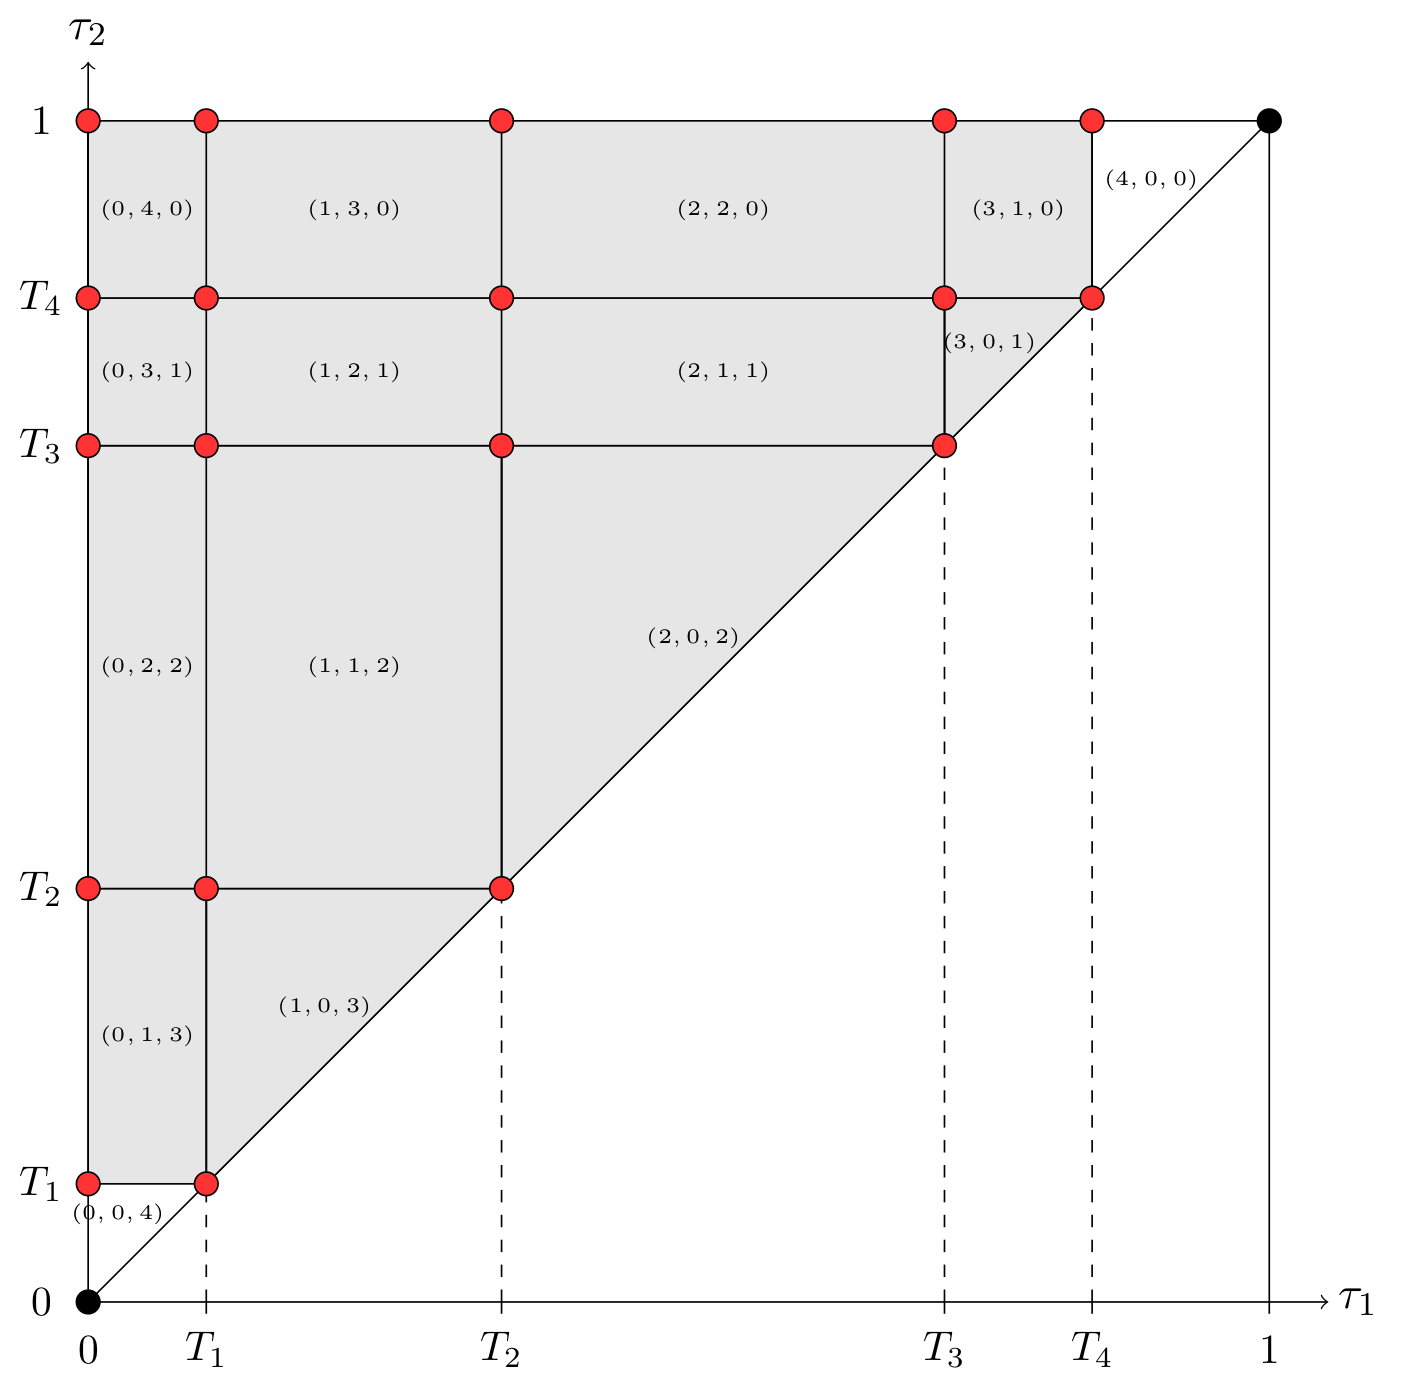
\includegraphics[width=0.35\textwidth]{space-partitioning}
    \caption{Partitionnement de l'espace de segmentation pour $K=3$ et $\tau = (\tau_1,\tau_2)$}
    \label{fig:space-partitioning}
\end{wrapfigure}

\section{Apport personnel}





% \begin{wrapfigure}{r}{0.35\textwidth}
%     <<'plot', eval = TRUE, fig = TRUE>>=
%     plot(Titanic)
%     @
%     \caption{Titanic plot}
% \end{wrapfigure}

\section*{Bibliographie}

\printbibliography
\nocite{*}

\end{document}
